\section{Exercício 1}

Considere o experimento computacional denominado “Polynomial Curve Fitting”, usado
diversas vezes no livro texto (veja páginas 4 e 5 do livro, bem como Apêndice A), considerando a
ordem do modelo sendo M = 9 e o tamanho da amostra sendo N = 10.
Faça:

\begin{enumerate}[label=(\alph*)]
    \item Calcule a solução de mínimos quadrados (LS) \( \mathbf{w_{LS}} \);
    \item Calcule a solução via regressão ridge (escolha um fator de regularização razoável) \( \mathbf{w_{ridge}} \);
    \item Calcule a solução via regressão lasso (escolha um fator de regularização razoável) \( \mathbf{w_{lasso}} \);
    \item Monte uma tabela exibindo os 10 coeficientes \( \mathbf{w} \) para as 3 soluções obtidas nos itens acima e comente/compare os resultados;
    \item Plote uma figura contendo o processo gerador em verde (a senoide), e suas estimativas \( y_{LS} \), \( y_{ridge} \), e \( y_{lasso} \) em preto, azul e vermelho, respectivamente;
    \item Repita todos os itens anteriores para \( N=20 \) e \( N=50 \).
\end{enumerate}

\subsection{Resposta do item (a)}
Para responder esse item foi utilizada a classe $LinearRegression()$ da biblioteca \textit{sklearn} para linguagem \textit{Python}, que realiza uma regressão linear utilizando mínimos quadrados. Foi escolhido um polinômio de ordem 9 como modelo.
\begin{figure}[H]
    \centering
    \caption{Solução para mínimos quadrados (LS)}
    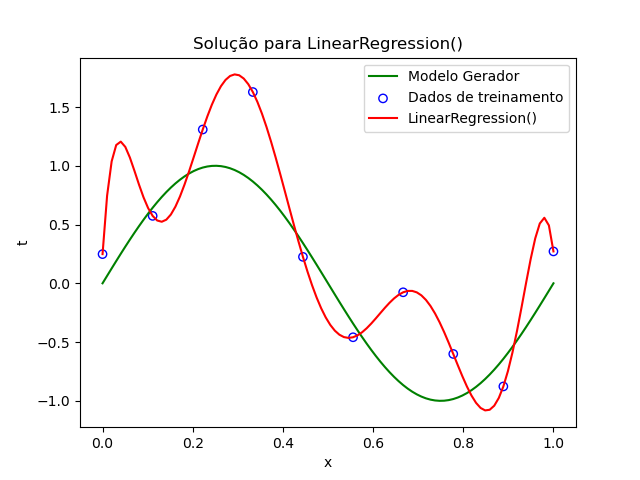
\includegraphics[width=12cm]{E1_a.png}
\end{figure}
A regressão linear por mínimos quadrados não introduz nenhuma regularização e por isso a curva vermelha passa exatamente pelos dados de treinamento, mostrando que eles foram decorados overfitting.


\subsection{Resposta do item (b)}
Para responder esse item foi utilizada a classe $Ridge()$ da biblioteca \textit{sklearn} para linguagem \textit{Python}, que realiza uma regressão linear utilizando mínimos quadrados e regularização de norma $L_2$ (Ridge). Foi escolhido um polinômio de ordem 9 como modelo e o fator de regularização $\lambda$, que na classe $Ridge()$ é chamado de \textit{alpha}, que melhor adaptou a curva ao modelo gerador foi $1^{-0.5}$.
\begin{figure}[H]
    \centering
    \caption{Solução para Ridge com $\lambda = 1^{-0.5}$}
    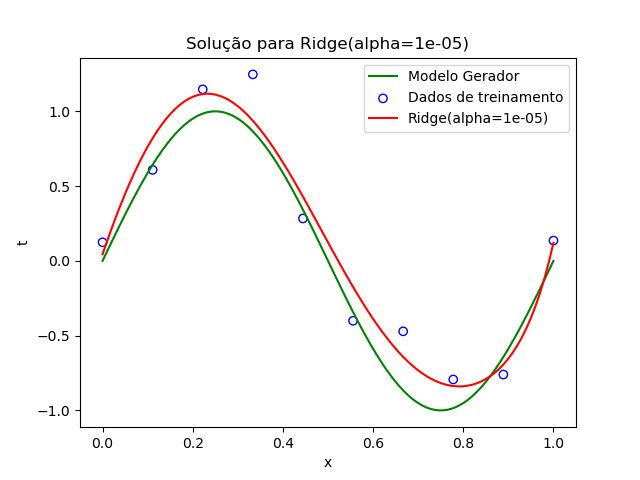
\includegraphics[width=12cm]{E1_b.png}
\end{figure}
A regressão Ridge introduz uma penalização nos coeficientes através do fator de regularização, ajudando a evitar overfitting.

\subsection{Resposta do item (c)}
Para responder esse item foi utilizada a classe $Lasso()$ da biblioteca \textit{sklearn} para linguagem \textit{Python}, que realiza uma regressão linear utilizando mínimos quadrados e regularização de norma $L_1$ (Lasso). Foi escolhido um polinômio de ordem 9 como modelo e o fator de regularização $\lambda$, que na classe $Lasso()$ é chamado de \textit{alpha}, que melhor adaptou a curva ao modelo gerador foi $1^{-0.5}$.
\begin{figure}[H]
    \centering
    \caption{Solução para Lasso com $\lambda = 10^{-0.6}$}
    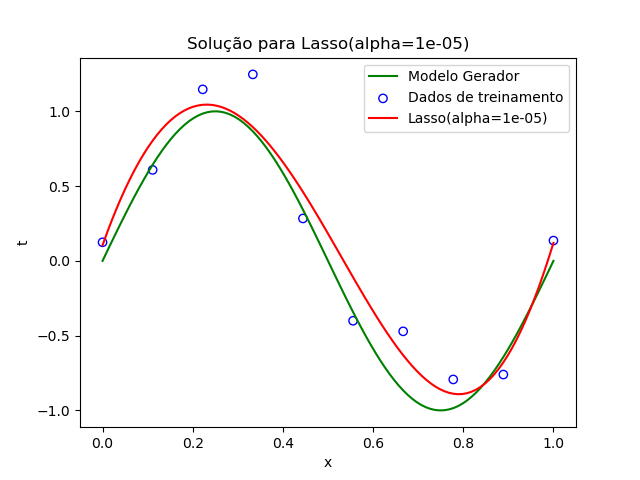
\includegraphics[width=12cm]{E1_c.png}
\end{figure}
A regressão Lasso, assim como a Ridge, introduz uma penalização nos coeficientes através do fator de regularização, ajudando a evitar overfitting.

\subsection{Resposta do item (d)}

A tabela abaixo exibindo os coeficientes para as três soluções permite comparar diretamente o impacto da regularização nos coeficientes.

\begin{table}[H]
\caption{Coeficientes para $N=10$}
\resizebox{\textwidth}{!}{
    \begin{tabular}{lllllllllll}
        \toprule
        Modelo & w0 & w1 & w2 & w3 & w4 & w5 & w6 & w7 & w8 & w9 \\
        \midrule
        LS & 0.00 & 61.35 & -1305.40 & 10864.20 & -43958.49 & 96013.73 & -116795.02 & 75859.90 & -22104.00 & 1363.74 \\
        Ridge & 0.00 & 5.58 & -10.39 & -3.32 & 2.25 & 3.46 & 2.37 & 0.81 & -0.28 & -0.58 \\
        Lasso & 0.00 & 7.87 & -18.23 & 2.99 & 5.02 & 2.16 & 0.11 & 0.00 & -0.00 & 0.09 \\
        \bottomrule
    \end{tabular}
}
\end{table}

A regressão por mínimos quadrados sem regularização tende a produzir coeficientes maiores, um dos sinais que indicam overfitting ou pelo menos uma alta sensibilidade aos dados de treinamento. Enquanto que os coeficientes produzidos pela Ridge e pela Lasso são menores.

Além disso, é possível observar a presença de alguns coeficientes praticamente nulos para a Lasso. Esse resultado era esperado, uma vez que a Lasso, por utilizar a norma $L_1$, tende a produzir uma solução mais esparsa, selecionando atributos mais importantes.

Enquanto isso, a regressão Ridge, apesar de não selecionar atributos como a Lasso, tende a penalizar ainda mais os coeficientes grandes, consequentemente fazendo com que os maiores coeficientes fiquem menores que os produzidos pela Lasso.



\subsection{Resposta do item (e)}
\begin{figure}[H]
    \centering
    \caption{Comparação entre as soluções para $N=10$}
    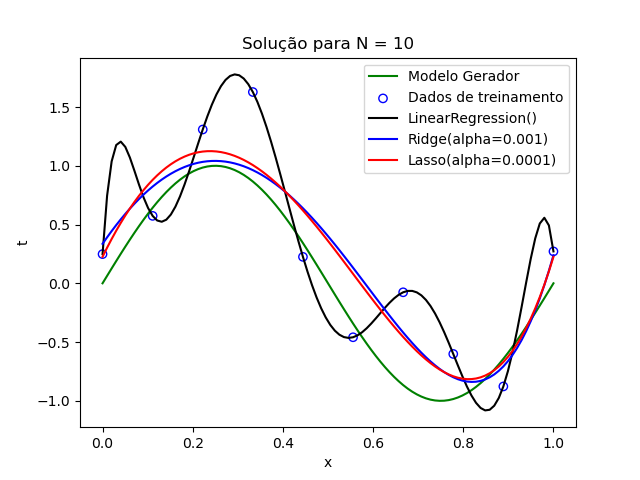
\includegraphics[width=12cm]{E1_e.png}
\end{figure}

\subsection{Resposta do item (f)}

\begin{figure}[H]
    \centering
    \caption{Comparação entre as soluções para $N=20$}
    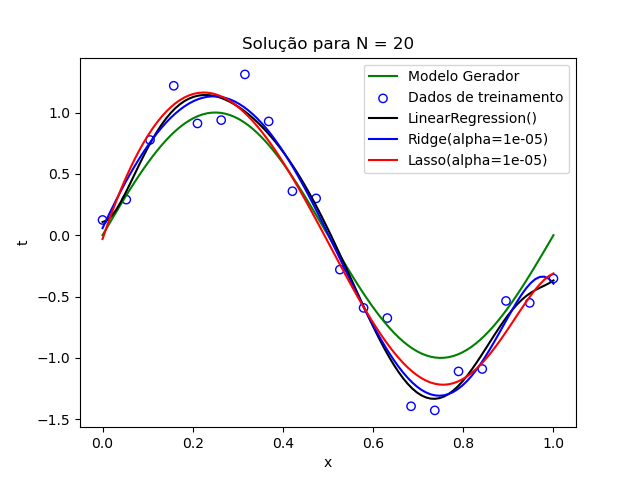
\includegraphics[width=12cm]{E1_f20.png}
\end{figure}
\begin{table}[H]
    \caption{Coeficientes para $N=20$}
    \resizebox{\textwidth}{!}{
        \begin{tabular}{lllllllllll}
            \toprule
            Modelo & w0 & w1 & w2 & w3 & w4 & w5 & w6 & w7 & w8 & w9 \\
            \midrule
            LS & 0.00 & -6.01 & 266.50 & -2042.90 & 7178.62 & -13245.77 & 11993.84 & -3017.56 & -2424.09 & 1296.42 \\
            Ridge & 0.00 & 8.39 & -16.21 & -8.40 & 2.98 & 9.30 & 9.76 & 5.62 & -1.60 & -10.66 \\
            Lasso & 0.00 & 12.42 & -29.59 & 0.72 & 10.39 & 8.98 & 4.55 & 0.00 & -1.36 & -6.72 \\
            \bottomrule
        \end{tabular}
    }
\end{table}

\begin{figure}[H]
    \centering
    \caption{Comparação entre as soluções para $N=50$}
    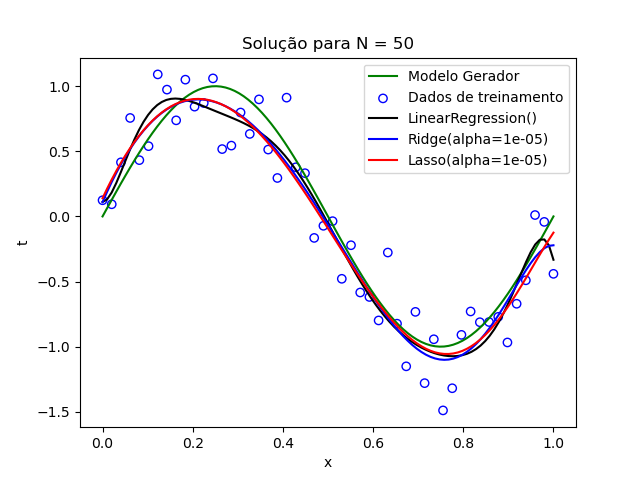
\includegraphics[width=12cm]{E1_f50.png}
\end{figure}
\begin{table}[H]
    \caption{Coeficientes para $N=50$}
    \resizebox{\textwidth}{!}{
        \begin{tabular}{lllllllllll}
            \toprule
            Modelo & w0 & w1 & w2 & w3 & w4 & w5 & w6 & w7 & w8 & w9 \\
            \midrule
            LS & 0.00 & -6.39 & 455.99 & -5270.52 & 27669.17 & -80097.05 & 135776.46 & -134351.92 & 71926.94 & -16103.56 \\
            Ridge & 0.00 & 4.21 & -10.54 & -3.23 & 1.84 & 4.62 & 5.21 & 3.53 & -0.31 & -6.02 \\
            Lasso & 0.00 & 5.12 & -14.48 & 0.36 & 4.73 & 4.19 & 2.22 & 0.00 & -0.00 & -2.74 \\
            \bottomrule
        \end{tabular}
    }
\end{table}

Pelas figuras, podemos observar que a solução para mínimos quadrados começa a sofrer menos com o overfitting à medida que o tamanho da amostra aumenta. Isso se deve ao fato de que o ruído nos dados de treinamento possui uma distribuição gaussiana com média zero. Pela lei dos grandes números, quanto maior a quantidade de dados de treinamento, mais a média da amostra se aproxima da média da distribuição original, que é zero, reduzindo assim o efeito do ruído.

Consequentemente, com mais dados, a solução de mínimos quadrados consegue capturar melhor o padrão subjacente dos dados, e o impacto do ruído diminui. Esse comportamento explica por que a solução de mínimos quadrados apresenta um ajuste mais estável e menos propenso ao overfitting quando o tamanho da amostra aumenta.

No entanto, é importante notar que, mesmo com um aumento no tamanho da amostra, métodos de regularização como a regressão ridge e lasso continuam a fornecer soluções mais robustas e generalizáveis, especialmente em situações onde o ruído pode não ser perfeitamente gaussiano ou quando a complexidade do modelo ainda é alta em relação ao tamanho da amostra.






